\documentclass[12pt,twoside,singlespace]{article}
\pagestyle{plain}

\usepackage{array, paralist, enumerate, amsmath, amsthm, amsfonts, amssymb, color, mathrsfs,comment}
%\usepackage{times}
\usepackage{geometry}
\usepackage{framed}
\usepackage{hyperref}
\usepackage{graphicx}
\usepackage{epstopdf}

\usepackage{tikz}
\usepackage{tkz-graph}
\usetikzlibrary{arrows,%
                shapes,positioning}

\definecolor{DarkBlue}{rgb}{0,0,0.8} 
\definecolor{DarkGreen}{rgb}{0,0.5,0.0} 
\definecolor{DarkRed}{rgb}{0.9,0.0,0.0} 

\usepackage[T1]{fontenc}
\usepackage[latin1]{inputenc}
%\usepackage[inline]{showlabels}

\numberwithin{equation}{section}
\newtheorem{thm}[equation]{Theorem}
\newtheorem{lem}[equation]{Lemma}
\newtheorem{cor}[equation]{Corollary}
\newtheorem{prop}[equation]{Proposition}

\theoremstyle{definition}
\newtheorem{definition}[equation]{Definition}
\newtheorem{ex}[equation]{Example}	
\newtheorem{remark}[equation]{Remark}
\newtheorem{prob}{Problem}
\newtheorem{construction}[equation]{Construction}

\newcommand{\BB}{\mathbf{B}}
\newcommand{\ZZ}{\mathbf{Z}}
\newcommand{\NN}{\mathbf{N}}
\newcommand{\RR}{\mathbf{R}}
\newcommand{\QQ}{\mathbf{Q}}
\newcommand{\CC}{\mathbf{C}}
\newcommand{\FF}{\mathbf{F}}
\newcommand{\N}{N}
\newcommand{\po}[2]{\mathfrak{po}^{#1|#2}}
\newcommand{\on}{\operatorname}
\newcommand{\ra}{\rightarrow}
\newcommand{\ul}{\underline}
\newcommand{\ol}{\overline}
\newcommand{\nin}{\noindent}

\newcommand{\simple}{\text{simple}}
\newcommand{\Img}{\on{Im}}
\newcommand{\con}{\on{Con}}
\newcommand{\dash}{\on{Dash}}

\geometry{verbose,letterpaper,tmargin=1in}

\newcommand{\Q}{\overline{q}}
\newcommand{\w}{\on{weight}}

\newcommand{\val}{\on{Val}}
\newcommand{\smon}{\mathbf{SMon}}
\newcommand{\clif}{\on{clif}}
\newcommand{\cl}{\mathbf{Cl}}
%\newcommand{\mov}[2]{\on{mov}_{#2}(#1)}
\newcommand{\inc}{\on{inc}}
\newcommand{\cut}[4]{#1 = #2 \amalg_{#4} #3}
\newcommand{\cutr}[3]{#1 \amalg_{#3} #2}
%\newcommand{\piece}[3]{#1(#2|#3)}
\newcommand{\piece}[3]{#1_{#3}}
\newcommand{\wt}{\on{wt}}

\newcommand{\com}[1]{\textcolor{red}{$[\star \star \star$ #1 $\star \star \star]$}}

%%%%%%%%%%%%%%%%%%%%%%%%%%%%%% LyX specific LaTeX commands.
%% Bold symbol macro for standard LaTeX users
\providecommand{\boldsymbol}[1]{\mbox{\boldmath $#1$}}

%%%%%%%%%%%%%%%%%%%%%%%%%%%%%% User specified LaTeX commands.
\renewcommand{\vec}[1]{\mathbf{#1}}

%\renewcommand{\labelenumi}{(\alph{enumi})}
%\renewcommand{\labelenumii}{(\roman{enumii})}

%\usepackage{babel}

\title{Strucutral Theory of 2D Adinkras}
\author{Kevin Iga and Yan X Zhang}

\begin{document}

\pagestyle{plain}

\maketitle

\begin{abstract}
Alternate Version of Main Theorem
\end{abstract}






\section{Every $2$-d Adinkra is a Quotient}
\label{sec:quotient}

In Section~\ref{sec:products}, we showed that we can construct a $2$-d Adinkra by a product construction of two $1$-d Adinkras, each of which appears on the boundary of the product. In this section, we settle a conjecture of H\"ubsch \cite{hubsch:weaving} by showing that every $2$-d Adinkra is in fact a quotient of the the product of the two $1$-d Adinkras on its lower boundary. Our main result is:

\begin{thm}
\label{thm:quotient}
Let $A$ be a connected $2$-d Adinkra.  Fix a vertex $\overline{0}$ in $A$ and let $A_L^0$ (resp. $A_R^0$) be the connected component of $A_L$ (resp. $A_R$) containing $\overline{0}$. Then the following hold:
\begin{enumerate}
\item[I] There is a binary block code $K$ of length $n$ so that $K\cap \hat{C}(A_L^0)=0$ and $K\cap \check{C}(A_R^0)=0$, and
\[C(A)=\hat{C}(A_L^0)\oplus \check{C}(A_R^0)\oplus K;\]
\item[II] there is a graph isomorphism
\begin{equation}
\label{eqn:quotientiso}
A\cong (A_L^0\times A_R^0)/K
\end{equation}
of the underlying graphs that preserves colors and the bigrading;
\item[III] there is a representative $A'$ in the same vertex switching class of $A_L^0\times A_R^0$ whose dashing is invariant under $K$, and the quotient by $K$ gives a dashing that agrees with the dashing on $A$ when compared via the isomorphism given in $(II)$. 
\end{enumerate}
\end{thm}

We first show parts $(I)$ and $(II)$ of this Theorem, starting with the codes. We delay the proof and relevant definitions of $(III)$ to after.

\begin{lem}
\label{lem:cplus}
\[\hat{C}(A_L^0)\oplus \check{C}(A_R^0) \subseteq C(A).\]
\end{lem}
\begin{proof}
Let $g\in\hat{C}(A_L^0)$ and $h\in \check{C}(A_R^0)$.  Then $g\overline{0}=\overline{0}$ because applying $g$ to $\overline{0}$ results in a path that lies completely inside $A_L^0$, and so the fact that $g\overline{0}=\overline{0}$ in $A_L^0$ (since $g\in \hat{C}(A_L^0)$) results in $g\overline{0}=\overline{0}$ in $A$.  Likewise $h\overline{0}=\overline{0}$.  So $(g+h)\overline{0}=g(h(\overline{0}))=\overline{0}$ and $g+h\in C(A)$.
\end{proof}

\begin{proof}[Proof of Theorem~\ref{thm:quotient}, $(I)$ and $(II)$]
From Lemma~\ref{lem:cplus} and basic linear algebra, there exists a vector subspace $K$ of $\ZZ_2^n$ that is a vector space complement of
$\hat{C}(A_L^0)\oplus \check{C}(A_R^0)$ in $C(A)$.  That is,
\[C(A)=\hat{C}(A_L^0)\oplus \check{C}(A_R^0)\oplus K.\]



As always, $\ZZ_2^n$ acts on $A_L^0\times A_R^0$ by color-preserving graph isomorphisms.  When this action is restricted to $K$, the action is faithful because $K\cap \hat{C}(A_L^0)\oplus \check{C}(A_R^0)=0$.  Since $K$ is a subgroup of $C(A)$, which is doubly even, we see that the action of $K$ is distant.  By Proposition~\ref{prop:quotient}, there is a well-defined graph quotient $(A_L^0\times A_R^0)/K$.


We now define a graph homomorphism
\[\Phi:A_L^0\times A_R^0 \to A\]
as follows.

Let $(v_1,v_2)\in A_L^0\times A_R^0$.  Then by Proposition~\ref{prop:transitive}, there is a word $\vec{x}_1\in \hat{\ZZ}_2^p$ so that $\vec{x}_1\overline{0}=v_1$ and a word $\vec{x}_2\in \check{\ZZ}_2^q$ so that $\vec{x}_2\overline{0}=v_2$.  We define $\Phi(v_1,v_2)=(\vec{x}_1+\vec{x}_2)\overline{0}$ in $A$.

The $\vec{x}_1$ and $\vec{x}_2$ are defined up to $\hat{C}(A_L^0)$ and $\check{C}(A_R^0)$, respectively.  Since $\hat{C}(A_L^0)$ and $\check{C}(A_R^0)$ are subgroups of $C(A)$, we see that the definition of $\Phi(v_1,v_2)$ does not depend on these choices.

\com{Describe action of $C(A)$ on $A_L^0\times A_R^0$.}

But actually by the same argument, for all $g\in C(A)$, $\Phi(g(v_1,v_2))=(v_1,v_2)$.  Therefore $\Phi$ actually acts on the quotient.



To show that this is onto, let $v$ be a vertex in $A$.  Since $A$ is connected, there is a word $\vec{x}\in \ZZ_2^n$ so that $\vec{x}\overline{0}=v$.  Let $\pi_1:\ZZ_2^n\to \ZZ_2^p$ and $\pi_2:\ZZ_2^n\to\ZZ_2^q$ be projection onto the first $p$ and last $q$ bits, respectively.  Let $v_1=\pi_1(\vec{x})\overline{0}$ in $A_L^0$ and $v_2=\pi_2(\vec{x})\overline{0}$ in $A_R^0$.  \com{Do we worry about ambiguity here that these are the last $q$ bits shifted to be in the range 1...q?}

Then $\Phi(v_1,v_2)=v$.

To show that this is one-to-one, suppose $(v_1,v_2)$ and $(v_3,v_4)$ are vertices in $A_L^0\times A_R^0$ and suppose $\Phi(v_1,v_2)=\Phi(v_3,v_4)$.  Define $\vec{x}_1$, $\vec{x}_2$, $\vec{x}_3$, and $\vec{x}_4$ as above, so that $\vec{x}_1\overline{0}=v_1$, and so on.  We then have $(\vec{x}_1+\vec{x}_2)\overline{0}=(\vec{x}_3+\vec{x}_4)\overline{0}$.  Then $(\vec{x}_1-\vec{x}_3+\vec{x_2}-\vec{x}_4)\overline{0}=\overline{0}$, so that $\vec{x}_1-\vec{x}_3+\vec{x}_2-\vec{x}_4\in C(A)$.  Let $\vec{y}=\vec{x}_1-\vec{x}_3+\vec{x}_2-\vec{x}_4$.  Since $C(A)=\hat{C}(A_L^0)\oplus \check{C}(A_R^0)\oplus K$, we can write $\vec{y}=\vec{y}_1+\vec{y}_2+\vec{y}_3$ where $\vec{y}_1\in \hat{C}(A_L^0)$, $\vec{y}_2\in \check{C}(A_R^0)$, and $\vec{y}_3\in K$.

Then since $\vec{y}_1\in \hat{C}(A_L^0)$, we have that $(\vec{x}_1+\vec{y}_1)\overline{0}=v_1$.  Likewise, since $\vec{y}_2\in\check{C}(A_R^0)$, we have $(\vec{x}_2+\vec{y}_2)\overline{0}=v_2$.  Then $\vec{y}_3 (v_1,v_2) = (v_3,v_4)$.

\com{This is awkward notation}
Take the $h_L(v_1,v_2)=h_1(v_1)$ and note that $h_L(\Phi(v_1,v_2))=h_1(v_1)$.  Likewise $h_R(\Phi(v_1,v_2))=h_2(v_2)$.



\end{proof}

Note that $\Phi(v,\overline{0})=v$ on $A_L^0\times\{\overline{0}\}$, and $\Phi(\overline{0},v)=v$ on $\{\overline{0}\}\times A_R^0$.








\begin{comment}




\begin{figure}[htb]
\begin{center}

\begin{tabular}{c|c}
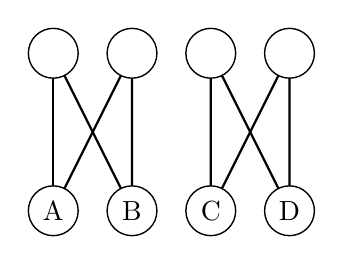
\begin{tikzpicture}[scale=0.10]
%\SetVertexNormal
\SetUpEdge[labelstyle={draw}]
\Vertex[x=0,y=0]{A}
\Vertex[x=10,y=0]{B}
\Vertex[x=20,y=0]{C}
\Vertex[x=30,y=0]{D}
\SetVertexNoLabel
\Vertex[x=0,y=20]{E}
\Vertex[x=10,y=20]{F}
\Vertex[x=20,y=20]{G}
\Vertex[x=30,y=20]{H}
\Edges(A, F, B, E, A)
\Edges(C, H, D, G, C)
\end{tikzpicture}
&
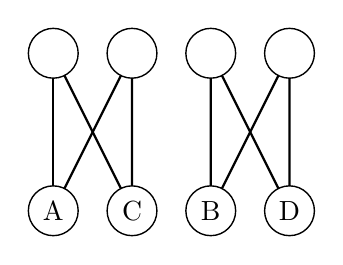
\begin{tikzpicture}[scale=0.10]
%\SetVertexNormal
\SetUpEdge[labelstyle={draw}]
\Vertex[x=0,y=0]{A}
\Vertex[x=10,y=0]{C}
\Vertex[x=20,y=0]{B}
\Vertex[x=30,y=0]{D}
\SetVertexNoLabel
\Vertex[x=0,y=20]{E}
\Vertex[x=10,y=20]{G}
\Vertex[x=20,y=20]{F}
\Vertex[x=30,y=20]{H}
\Edges(A, G, C, E, A)
\Edges(B, H, D, F, B)
\end{tikzpicture}
\end{tabular}
%\includegraphics[scale=0.5]{4cubefold}
\caption{Taking the product of the two adinkras here with the following identification gives a non-disconnected adinkra with 16 vertices. \label{fig:disconnected}}
\end{center}
\end{figure}

\end{comment}

Unfortunately, it is too much to expect the dashing on $A_L^0\times A_R^0$ to agree with the dashing on $A$; it is also almost always false that the dashing on $A_L^0\times A_R^0$ is invariant under the quotienting action of $K$. However, if we allow the operation of \emph{vertex switching}, then we can basically accomplish these goals, giving part $(III)$ of Theorem~\ref{thm:quotient}.

\begin{definition}[Vertex switching]
Given an Adinkra $A$ (either $1$-d or $2$-d), and a vertex $v$ of $A$, we define \emph{vertex switching at $v$} to be the operation on $A$ that returns a new Adinkra $A'$ with the same vertices, edges, coloring, and grading(s) but a new dashing $\mu'$ so that
\begin{equation}
\mu'(e)=\begin{cases}
1-\mu(e),&\mbox{if $e$ is incident to $v$}\\
\mu(e),&\mbox{otherwise.}
\end{cases}
\end{equation}
Vertex switching induces a partition of dashings on $A$ into equivalence classes; call these \emph{vertex switching classes} of $A$.
\end{definition}

\begin{prop}
\label{prop:switching-still-adinkra}
If $A$ is an Adinkra, then so is $A'$.
\end{prop}
\begin{proof}
Since the vertices, edges, coloring, and grading(s) are the same, the only thing to check is the admissibility of $\mu'$.  That is, given colors $c_1$ and $c_2$, and vertices $v$, $w$, $x$, and $y$, such that $(v,w)$ and $(x,y)$ are edges with color $c_1$ and $(w,x)$ and $(y,v)$ are edges with color $c_2$, that $\mu'(v,w)+\mu'(w,x)+\mu'(x,y)+\mu'(y,v)$ is odd.  If $v'$ is none of these vertices, then this sum is unchanged.  If $v'$ is any of these vertices, for instance, $v$, then $\mu'(v,w)$ and $\mu'(y,v)$ are both changed modulo $2$, so that the sum modulo $2$ is still unchanged.
\end{proof}

Douglas, Gates, and Wang \cite{douglas} examined dashings in adinkras from a point of view inspired by Seidel's \emph{two-graphs} \cite{seidel:survey} \footnote{In Seidel's setting, \emph{vertex switching} switched the existence of edges, not the sign of edges; this can be seen as equivalent our definition applied to the complete graph. The type of vertex switching we do in this paper is sometimes called vertex switching on \emph{signed graphs}, to disambiguate from Seidel's usage.}. The second author \cite{zhang:adinkras} enumerated vertex switching classes and the number of dashings of $1$-d Adinkras. In this work, we use vertex switchings again to study $2$-d Adinkras.

Consider the dashing $\mu$ on $A$.  This restricts to $A_L^0$ and $A_R^0$, and Construction~\ref{const:product} produces a dashing $\mu_1$ on $A_L^0\times A_R^0$. At the same time, under the isomorphism (\ref{eqn:quotientiso}), the dashing $\mu$ on $A$ gets carried to $(A_L^0\times A_R^0)/K$.  The graph homomorphism
\[\pi:A_L^0\times A_R^0\to (A_L^0\times A_R^0)/K\]
pulls back the dashing to $\mu_2$ on $A_L^0\times A_R^0$. While $\mu_1$ and $\mu_2$ are fairly different, they agree on the ``lower boundary:''

\begin{lem}
\label{lem:agree-on-boundary}
The dashings $\mu_1$ and $\mu_2$ agree on $A_L^0\times \{\overline{0}\}$ and on $\{\overline{0}\}\times A_R^0$.
\end{lem}
\begin{proof}
The construction of $\mu_1$ gives all edges in $A_L^0\times\{\overline{0}\}$ as the same as in $A_L^0$ under the association of every edge $(v,w)$ with $((v,\overline{0}),(w,\overline{0}))$.  For $\mu_2$, the graph homomorphism $\Phi:A_L^0\times A_R^0\to A$ sends $(v,\overline{0})$ to $v$ for all $v\in A_L^0$ and $(\overline{0},v)$ to $v$ for all $v\in A_R^0$.  So $\mu_2$ on $A_L^0\times \{\overline{0}\}$ and $\{\overline{0}\}\times A_R^0$ is the same as $\mu_1$.
\end{proof}

Note that part $(III)$ of Theorem~\ref{thm:quotient} can be reformulated as saying that $\mu_1$ and $\mu_2$ are equivalent under vertex switching. Our strategy will be to reduce the problem to checking a set of local conditions on cycles. We now give some definitions and auxiliary results for our approach.


\begin{lem}
\label{lem:cycles-switching-class}
Two dashings have the same parity on all cycles\footnote{This type of result has a natural reformulation with homological algebra, done in independent ways by the first author's work using cubical cohomology \cite{dil:cohomology} and the second author's work using CW-complexes \cite{zhang:adinkras}. In either formulation, having parities of $\mu_1$ and $\mu_2$ agree on cycles is equivalent to $\mu_1 = \mu_2 = 0$ in cohomology.} if and only if they belong to the same vertex switching class.
\end{lem}

\begin{proof}
Let the dashings be $\mu$ and $\mu'$ on the Adinkra $A$. Since vertex switching preserves parity on any cycle, the ``if'' direction is trivial and it suffices to prove the other direction.

Assume $\mu$ and $\mu'$ have the same parity on all cycles. It suffices to prove the statement for $A$ connected, since we can repeat our argument on each connected component of $A$. Pick a spanning tree $T$ of $A$, and pick a vertex $v$ of $A$ to serve as the root. The choice of $v$ induces a map $d$ on the vertices of $A$ that associates to each vertex its distance from $v$ using just edges in $T$ (so $d(v) = 0$), which in turn induces a map on the edges of $T$ by associating to each edge $(x,y)$ the min of $d(x)$ and $d(y)$ (these two values are necessarily $1$ apart). We denote this value $d(x,y)$, which gives a partial ordering on the edges of $T$, which we also call $d$ by slight abuse of notation; to be precise, $d((x,y)) < d((x,y))$ in the ordering $d$ whenever $d(x,y) < d(x,y)$ in the edge function $d$.

Now, extend $d$ to a total ordering $d'$ on the edges of $T$. We claim that we can vertex switch $\mu$ such that $\mu$ agrees with $\mu'$ on $T$. Take the minimal edge $e$ (under $d'$) where the two dashings differ. $e = (x,y)$, where without loss of generality $d(y) > d(x)$. Note that vertex switching at $y$ cannot change the dashing on any of the edges $e < e'$ under the ordering $d'$, since otherwise $d(y)$ should have been assigned a smaller value. Thus, we can greedily vertex switch to make $\mu$ and $\mu'$ equal on $T$.

Finally, if $\mu$ and $\mu'$ are equal on $T$, consider any edge $e$ not in $T$. This edge completes at least one cycle with edges in $T$ (otherwise $T$ was not a minimal spanning tree). Since the two cycles have the same parity in $\mu$ and $\mu'$ by assumption and the dashings agree on all edges but $e$, $e$ must be dashed in the same way under the two dashings. Thus, the two dashings must actually agree on all edges, meaning the two original dashings are in the same vertex switching class.
% However, since $\mu$ and $\mu'$ agree on all cyclesminimal cycles, they agree on all cycles by Lemma~\ref{lem:minimal-cycles-to-all-cycles}, and in particular this cycle. 

\end{proof}

In light of the above Lemma, it suffices for us to prove that the parities of $\mu_1$ and $\mu_2$ agree on all cycles of $A_L^0\times A_R^0$:

\begin{proof}[Proof of Theorem~\ref{thm:quotient}, $(III)$]
Let our cycle be $(v_0,v_1,\ldots,v_k)$ with $v_0=v_k$. We first consider the case where $v_0=\overline{0}$.  Then there is a color sequence $\sigma$ from this.  We modify the path (and thereby modify the color sequence) by ``bubble sorting'' the colors.  Earlier, we noted that we could rearrange $\sigma$ to $l(\sigma)$ so that the left-moving colors were before the right-moving colors.  This can be more specifically done by a series of adjacent swaps of the type that sends the color sequence
\[(i_1,\ldots,i_{j-1},i_j,i_{j+1},i_{j+2},\ldots,i_k)\]
to
\[(i_1,\ldots,i_{j-1},i_{j+1},i_j,i_{j+2},\ldots,i_k).\]
A color swap of this type leads to a new path from $\overline{0}$, via Proposition~\ref{prop:colorpath}.  The path is unchanged up to $v_{j-1}$, but by the definition of Adinkras, property 3, the path returns to $v_{j+1}$ so it is only $v_j$ that has changed.  The effect on the parity of any dashing is, by property 3, to add $1$ modulo $2$.  In particular, $\mu_1$ and $\mu_2$ are both affected in the same way.

After a series of such color swaps, we rearrange $\sigma$ to $l(\sigma)$, and the path in question consists of left-moving edges, which remain in $A_L^0\times \{\overline{0}\}$, and then right-moving edges, which ends in $\overline{0}$, and so must be in $\{\overline{0}\}\times A_R^0$.  By Lemma~\ref{lem:agree-on-boundary}, $\mu_1$ and $\mu_2$ are equal here, and so their parity on this modified path is the same.  Therefore, their parity on the original loop was the same.

Now we consider loops $p$ where $v_0\not=\overline{0}$.  Since $A_L^0\times A_R^0$ is connected, there is a path $p_0$ from $\overline{0}$ to $v_0$.  Take the path $p_0$, followed by $p$, then followed by $p_0^{-1}$ (meaning $p_0$ traversed in the opposite sense).  This is a loop starting and ending in $\overline{0}$, but the parity of a dashing is the same as that of $p$, since every new edge in $p_0$ is counterbalanced by a new edge in $p_0^{-1}$.  Therefore the parity of $\mu_1$ and $\mu_2$ agree on all loops.
\end{proof}

 \com{This is the only place now where we refer to color sequences in any substantial way that is not subsumed by \ref{prop:reorderpath}.}
 
Theorem~\ref{thm:quotient} tells us that our quotient (which did not, a priori, play well with dashing) respects dashing if we allow the action of vertex switching; an alternative interpretation is that dashings should really be thought of as equivalence classes.

\begin{comment} % isn't this already proved?

\begin{lem}
\label{lem:minimal-cycles-to-all-cycles}
The set of parities on all cycles of an Adinkra $A$ are determined by parties on minimal (under inclusion) cycles of $A$.
\end{lem}
\begin{proof}
Consider a cycle in a graph as a $\mathbb{F}_2$-vector space over the edges of the graph. It is easy to check that any cycle $C$ is then a sum (as vectors in this vector space) of minimal cycles $C_1, \ldots, C_k$ and the parity of $C$ under a dashing is the sum of the parities of the minimal cycles $C_i$: each dashed edge in the $C_i$'s either appears twice and thus contributes $0$ to the parity (in which case it was not in $C$) or appears once and thus contributes $1$ to the parity (in which case it was in $C$). 
\end{proof}



\begin{proof}
Thanks to Proposition~\ref{prop:product-admissable}, we know that $\mu_1$ is admissable; we now show that $\mu_2$ is admissable as well. What we must prove is the following: given colors $c_1$ and $c_2$, and vertices $v$, $w$, $x$, and $y$, with edges $(v,w)$, $(w,x)$, $(x,y)$, and $(y,v)$ and colors $c(v,w)=c(x,y)=c_1$ and $c(w,x)=c(y,v)=c_2$, we have $\mu_2(v,w)+\mu_2(w,x)+\mu_2(x,y)+\mu_2(y,v)\equiv 1 \pmod{2}$.

Since $\pi$ is a graph homomorphism, and $c_1$, $c_2$, $v$, $w$, $x$, and $y$ are as above, then $\pi(v)$, $\pi(w)$, $\pi(x)$, and $\pi(y)$ satisfy the same condition.  If $\mu_2=\pi^*(\mu)$, then $\mu_2(v,w)+\mu_2(w,x)+\mu_2(x,y)+\mu_2(y,v)=\mu(\pi(v,w))+\mu(\pi(w,x))+\mu(\pi(x,y))+\mu(\pi(y,v))$ and the result follows from the fact that $\mu$ is an admissible dashing.


\end{proof}
\end{comment}


\section{ESDE Codes}

We have shown that each $2$-d Adinkra is constructed from a pair of $1$-d Adinkras plus a code; it is natural to ask which codes can appear. In this section, we classify these codes, which is another part of the conjectures of H\"ubsch \cite{hubsch:weaving}. 

\begin{definition}[Weights, ESDE codes]
Let $p$ and $q$ be non-negative integers so that $p+q=n$. For any $S \subset [n]$ and every element $\vec{x} \in \ZZ_2^n$, define $\wt_S(\vec{x})$ to be the number of $1$'s in the places corresponding to $S$; so in particular, $\wt_{[n]} = \wt$ as functions. Define an \emph{ESDE (even-split doubly-even) code of length $(p,q)$} to be a doubly-even code of length $n$ and a partition $L \cup R = [n]$ such that $|L| = p$, $|R| = q$, and every word $\vec{x}$ in the code has both $\wt_L(\vec{x})$ and $\wt_R(\vec{x})$ be even-valued. For our work, we always assume that $L = \{1, 2, \ldots, p\}$ and $R = \{p+1, p+2, \ldots, n\}$, since we can permute the indices without changing the structure of the code.
\end{definition}

We remark that ESDE codes are no more restrictive than doubly-even codes; an illustrative example is that any doubly-even code can be made into an ESDE code trivially by assigning $(p,q) = (n, 0)$ or $(0, n)$. This corresponds to the fact that any $1$-d Adinkra is trivially a $2$-d Adinkra with all colors left-moving or all colors right-moving. The main data in ESDE codes is the splitting. In fact, they are quite easy to classify:

\begin{prop}
\label{prop:esde}
Given a doubly-even $[n,k]$-code $C$, there is a bijection between codewords in $C^\perp$ and (ordered) paritions $L \cup R$ that make $C$ into an ESDE. There are $2^{n-k}$ such partitions. 
\end{prop}

\begin{proof}
Consider a partition $L \cup R$ that makes $C$ into an ESDE, and consider the codeword $w$ that is defined to have $1$ at all the positions in $L$ and $0$ at all the positions in $R$. By definition of ESDE codes, all codewords in $C$ have an even number of $1$'s in the support of $w$, which is equivalent to saying that $w$ is orthogonal to all the codewords in $C$. Thus, $w \in C^\perp$. Conversely, for any $w \in C^\perp$, $w$ is orthogonal to all codewords in $C$ and thus give an ESDE. Thus, there is a bijection between the two sets. Note these are ordered partitions; the codeword which has $1$ at all the positions in $R$ and $0$ otherwise would give the same paritition, but in reversed order.
\end{proof}


Recall \com{give citation once Kevin decides which theorems to use} that $1$-d chromotopologies are in bijection with quotients of the Hamming cube $I^n$ by a doubly-even code $K$, so any adinkra $A$ has a well-defined associated code $C(A)$ that is uniquely determined by just the graph structure of the adinkra. Our goal is to show that ESDE codes are exactly the codes that appear for $2$-d adinkras.

In \com{[references]}, there was a class of $1$-d Adinkras that were particularly easy to construct and study, called {\em Valise} Adinkras, whose height function had values in two adjacent integers (usually $0$ and $1$).  By analogy, given a ESDE code, we construct a $2$-d Adinkra called the {\em Valise 2-d Adinkra} that has support in a $2\times 2$ square.


\begin{construction}
\label{cons:valise}
Let $K$ be an ESDE code.  We will describe a construction that provides a $2$-d Adinkra with code $K$, called the {\em Valise 2-d Adinkra}. First, since $K$ is doubly-even, there exists a connected $1$-d Adinkra $A$ with code $C(A) = K$. \com{ [reference: this was a construction somewhere else]} Fix a vertex $\overline{0}$ of $A$. Now every vertex $v$ corresponds to a vector $\vec{v} \pmod{K}$. Define $h_L(v) = \wt_L(\vec{v}) \pmod{2}$ and $h_R(v) = \wt_R(\vec{v}) \pmod{2}$. Note that these functions are well-defined since $K$ is ESDE. $(h_L, h_R)$ gives a bigrading to $A$, making it a $2$-d Adinkra. % Note t, h_R(v)) =    For every vertex $v$ of $A$, pick a path from $\overline{0}$ to $v$.  This produces a color sequence $d$.  Define $h_L(v)$ to be the number $\pmod{2}$ of left-moving colors in $d$ and likewise $h_R(v)$ is the number modulo 2 of right-moving colors in $d$.  These functions are well-defined if every path from $\overline{0}$ to $v$ has the same parity in number of left-moving colors and in number of right-moving colors.  This occurs if and only if every loop starting from $\overline{0}$ has an even number of left-moving colors and an odd number of right-moving colors.  If $K$ is ESDE, then this is the case.
\end{construction}

\begin{figure}[htb]
\begin{center}

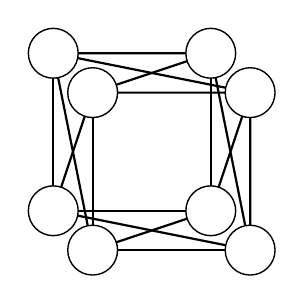
\begin{tikzpicture}[scale=0.10]
%\SetVertexNormal
\SetVertexNoLabel
\SetUpEdge[labelstyle={draw}]
\Vertex[x=0,y=0]{A}
\Vertex[x=-5,y=5]{H}
\Vertex[x=0,y=20]{C}
\Vertex[x=-5,y=25]{B}
\Vertex[x=15,y=5]{D}
\Vertex[x=20,y=0]{E}
\Vertex[x=20,y=20]{G}
\Vertex[x=15,y=25]{F}
\Edges(A,B,G)
\Edges(B,H,C)
\Edges(G,D)
\Edges(C,A,D,H,E,A)
\Edges(D,F,C,G,E,F,B)
\end{tikzpicture}
\caption{A valise $2$-d adinkra that cannot be put into non-valise form.\label{fig:tight valise}}
\end{center}
\end{figure}

\begin{thm}
\label{thm:esde}
For a code $K \subset \ZZ_2^n$, there exists a $2$-d adinkra $A$ with $C(A) = K$ if and only if $K$ is a ESDE code.
\end{thm}
\begin{proof}
Suppose $C(A) = K$ for some $2$-d Adinkra $A$. We know that $K$ is doubly-even. Consider any codeword $\alpha \in K$. Starting at $\overline{0} \in A$, moving by a path corresponding to $\alpha$ must end up back at $\overline{0}$. In particular, it must use an even number of left-moving (resp. right-moving) edges since each of such edge changes the $h_L$ (resp. $h_R$) by $1$ in absolute value. Thus, $C$ must be ESDE. 

Conversely, given an ESDE code $K$, we can use Construction~\ref{cons:valise} to get a $2$-d Adinkra with code $K$. By construction, $A$ is a $1$-d Adinkra with code $K$.  The only thing left to check is whether the $h_L$ and $h_R$ that are defined satisfy the correct properties on edges. Let $(v,w)$ be a left-moving edge in the Adinkra $A$.  Then the color of the edge is left-moving and so $h_L(v)\not=h_L(w)$ and $h_R(v)=h_R(w)$.  Since the possible values for $h_L$ and $h_R$ are $0$ and $1$, it follows that $|h_R(v)-h_R(w)|=1$. The proof is similar for right-moving edges.

\end{proof}

Given a $2$-d Adinkra $A$, with special basepoint $\overline{0}$ and corresponding $A_L^0$ and $A_R^0$, there remains the question of finding the code $K$.  Recall that
\[C(A)=\hat{C}(A_L^0)\oplus\check{C}(A_R^0)\oplus K.\]
There is some choice involved in defining $K$; it merely has to be a vector space complement to
\[C'=\hat{C}(A_L^0)\oplus\check{C}(A_R^0).\]
$K$ will more naturally be defined as $C(A)/C'$, though computationally we can choose a representative to be $K$.


Let $V^0=A_L^0\cap A_R^0$.  Now for every $v\in V^0$, we have $h_L(v)=h_L(\overline{0})$ and $h_R(v)=h_R(\overline{0})$ so in particular, $V^0$ has no edges; only vertices.

We construct a bijection between $V^0$ and $C(A)/C'$.

\begin{construction}
\label{cons:findk}
For every $v\in V^0$, there is a path $p_L$ from $\overline{0}$ to $v$ in $A_L^0$ and a path $p_R$ from $v$ to $\overline{0}$ in $A_R^0$.  These paths give color sequences $\sigma_L$ and $\sigma_R$ with $\beta_L=s(\sigma_L)$ and $\vec{x}_R=s(\sigma_R)$ so that $\vec{x}_L$ is $0$ in the last $q$ coordinates and $\vec{x}_R$ is $0$ in the first $p$ coordinates.  Since the paths $p_L$ and $p_R$ form a loop in $A$, we know that $\vec{x}_L+\vec{x}_R\in C(A)$.

The paths $p_L$ and $p_R$ are not canonical, but if $p'_L$ and $p'_R$ are other paths with those properties, then $p_L(p'_L)^{-1}$ is a loop in $A_L^0$ from $\overline{0}$.  Let $\sigma'_L$ and $\sigma'_R$ be the corresponding color sequences, then $s(\sigma_L)+s(\sigma'_L)\in C(A_L^0)$.  Likewise, $s(\sigma_R)+s(\sigma'_R)\in C(A_R^0)$.

Thus, the choice of $\vec{x}_L+\vec{x}_R$ is well-defined modulo $C'=\hat{C}(A_L^0)\oplus \check{C}(A_R^0)$.  This provides a map from $V^0$ to $K=C(A)/C'$.
\end{construction}

\begin{thm}
\label{thm:findk}
The above construction provides a bijective map
\[\Phi:V^0\to C(A)/C'\]
\end{thm}
\begin{proof}

We now prove this map is bijective by providing its inverse.  Suppose $\vec{x}\in C(A)$.  Then by Proposition~\ref{prop:colorpath}, there is a loop in $A$ starting at $\overline{0}$ that follows the colors indicated by $\vec{x}$.  By Proposition~\ref{prop:reorderpath}, there is a left-moving path $p_L$ from $\overline{0}$ to a vertex $v$, and a right-moving path $p_R$ from $v$ to $\overline{0}$.  Since $p_L$ is left-moving, $v\in A_L^0$.  Since $p_R$ is right-moving, $v\in A_R^0$.  Therefore $v\in V^0$.

Note that $v$ does not depend on the order of the left-moving colors in the color sequence, as long as they all come before the right-moving colors.  Thus we have a map
\[\Psi: C(A)  \to V^0.\]

Now suppose $\vec{y}\in \hat{C}(A_L^0)$ and $\vec{z}\in \check{C}(A_R^0)$.  We consider how the loop in the previous paragraph changes if we replace $\vec{x}$ with $\vec{x}+\vec{y}+\vec{z}$.  We use Proposition~\ref{prop:colorpath} to create a loop $p_1$ in $A_L^0$ that starts at $\overline{0}$ and follows the colors indicated by $\vec{y}$.  Then let $p_2$ be the path from $\overline{0}$ following the colors indicated by $s(\alpha)$ and $p_3$ the path that continues this using $s(\beta)$.  Finally, let $p_4$ be the path from there using the colors of $\vec{z}$.  By Proposition~\ref{prop:colorpath}, since $p_2$ starts from $\overline{0}$, it must still end at the same point $v$.  Therefore the map $\Psi$ descends to a map
\[\tilde{\Psi}:C(A)/C' \to V^0.\]

We now show that this function is the inverse of Construction~\ref{cons:findk}.  Let $v\in V^0$.  The construction gives a path $p_L$ of left-moving edges starting from $\overline{0}$ and ending in $v$ and a path $p_R$ of right-moving edges starting from $v$ to $\overline{0}$.  Composing these paths gives the result of the Construction.  Then we apply $\tilde{\Psi}$.  This takes the code word and finds the loop, which by Proposition~\ref{prop:colorpath} must be $p_Lp_R$.  Then $\Psi$ of the code word is the vertex at the end of $p_L$, which is $v$.

\com{This is a bit messy.  Clean it up}

[show the other composition is the identity]

\end{proof}

\section{Enumerating $2$-d Adinkras}
As a final illustration that we have characterized all $2$-d Adinkras, note that the constructions so far suffice to enumerate all $2$-d Adinkras.

\begin{construction}
First choose an ESDC code $C$.  Let $\pi_L:\ZZ_2^n\to\ZZ_2^p$ and $\pi_R:\ZZ_2^n\to\ZZ_2^q$ be projections onto the first $p$ and last $q$ bits, respectively.

Use the construction from \cite{rAT2} to create the $1$-d Adinkra $A=I^n/C$ with code $C$.  Use the splitting of $[n]$ to designate some edges left-moving and the others, right-moving.  Fix a vertex $\overline{0}$ in $A$.  Let $A_L^0$ and $A_R^0$ be as above. \com{Refer to specific construction}  Use the ``hanging gardens'' construction in Ref.~\cite{hgt} on $A_L^0/\pi_L(C)$ and pull it back to $A_L^0$ to create a height function $h_L$ on $A_L^0$ that is invariant under $\pi_L(C)$.  Likewise create a height function $h_R$ on $A_R^0$ invariant under $\pi_R(C)$.

Now extend $h_L$ on the rest of $A$ as follows: for every vertex $v$ of $A$, pick a path from $\overline{0}$ to $v$.  Use Proposition~\ref{prop:reorderpath} to obtain a left-moving path from $\overline{0}$ to a vertex $w$, and a right-moving path from $w$ to $v$.  Then $w\in A_L^0$ and define $h_L(v)=h_L(w)$.

Likewise define $h_R$ on $A$.
\end{construction}

The fact that the result is a $2$-d Adinkra follows from the following results.

\begin{lem}
The gradings $h_L$ and $h_R$ defined above are independent of the paths $p$ and $q$.\label{lem:indep}
\end{lem}

\begin{proof}
We first prove that $h_L$ is independent of the particular paths $p$ and $q$.  Suppose $p'$ is a left-moving path from $\overline{0}$ to $w'$ and $q'$ is a right-moving path from $w'$ to $v$.  Then $-p$ followed by $p'$ forms a left-moving path from $w$ to $w'$, and $q'$ followed by $-q$ forms a right-moving path from $w'$ to $w$.  These two paths form a cycle and so give an element of $C$.  The left-moving path from $w$ to $w'$ gives an element of $\pi_L(C)$.  Since $h_L$ is invariant under $\pi_L(C)$, we have that $h_L(w)=h_L(w')$.

Therefore $h_L(v)$ is independent of the path chosen.  Likewise $h_R(v)$ is also independent of the path chosen.
\end{proof}

\begin{lem}
If $v$ and $v'$ are vertices and $(v,v')$ is a left-moving edge, then
$|h_L(v)-h_L(v')|=1$ and $h_R(v)=h_R(v')$.  If $(v,v')$ is a right-moving edge, then $|h_R(v)-h_R(v')|=1$ and $h_L(v)=h_L(v')$.
\end{lem}

\begin{proof}
Let $v$ and $v'$ be vertices connected by an edge.  Fix a left-moving path $p$ from $\overline{0}$ to a vertex $w$ in $A_L^0$ and a right-moving path $q$ from $w$ to $v$.  Then $h_L(v)=h_L(w)$.

Suppose the edge $(v,v')$ is a right-moving edge.  By appending to $q$ the edge $(v,v')$, we have a right-moving path from $w$ to $v'$.  By Lemma~\ref{lem:indep}, we have $h_L(v)=h_L(v')$.

Now suppose the edge $(v,v')$ is a left-moving edge.  Let the color of this edge be $i$.  Let $w'=q_i(w)$.  The map $q_i$ is a graph isomorphism that sends the path $q$ to a new right-moving path $q'$ that connects $w'$ to $v'$.

Since there is a left-moving path from $\overline{0}$ to $w'$ (consisting of $p$ appended with an $i$-colored edge) and a right-moving path from $w'$ to $v'$, we know that $h_L(w')=h_L(v')$.  

Since there is a left-moving edge between $w$ and $w'$, we have $|h_L(w)-h_L(w')|=1$.  Since $h_L(w')=h_L(v')$ and $h_L(w)=h_L(v)$, we conclude that $|h_L(v)-h_L(v')|=1$.

The other cases can be obtained by symmetry.
\end{proof}


\begin{thm}
Every $2$-d Adinkra can obtained by this construction.
\end{thm}

\begin{proof}
Given any $2$-d Adinkra $A$, there is an ESDC code $C$.  Pick a vertex $\overline{0}$ and define $A_L^0$ and $A_R^0$ as in (\ref{thm}).

Restrict the gradings $h_L$ and $h_R$ onto $A_L^0$ and $A_R^0$.  Note that if $g\in C$, then $\pi_L(g)v=\pi_R(g)v$, and so $h_L(\pi_L(g)v)=h_L(v)$ and $h_R(\pi_L(g)v)=h_R(v)$.  Therefore $h_L$ restricted to $A_L^0$ is invariant under $\pi_L$.  Likewise $h_R$ restricted to $A_R^0$ is invariant under $\pi_R$.

The dashings, as described in \cite{rAT2}, can be obtained by choosing the specific quotient $I^n/C$.

Theorem~\ref{thm:main} gives a description of $A$ in terms of this construction.

\end{proof}

\bibliographystyle{abbrv}
\bibliography{Adinkras}





\end{document}